\section{Decentralisation}
    So far the system we have described might appear very centralised: we have a fixed number of nodes gossiping to decide the state of the network. This is a permissioned system, no one can join the network without permission. To decentralise the network, it is essential to make the system permissionless allowing anyone to join the network. To achieve this, Tagion uses \textit{swapping} to dynamically rotate nodes in and out of the Hashgraph.

\subsection{Node Pools}
    To ensure scalability as the system grows, Tagion maintains a constant number of nodes in the Hashgraph. While such a network consisting of a fixed set of nodes offer greater decentralisation than standard systems, it can never claim true decentralisation. True decentralisation eliminates central points of control, distributing power across a continuously changing network of participants. The network thus needs to be permissionless. Rather than adjusting the size of the Hashgraph as nodes want to join and leave the network, Tagion employs the notion of an active and a passive pool. The active pool is of constant size, and it is purely nodes within this pool that participate in the Hashgraph consensus protocol. In contrast, the passive pool does not influence the consensus, and dynamically adjusts in size to accommodate nodes joining or leaving the system. The passive pool allows a permissionless way to join the network.

\begin{figure}[H]
	\centering
	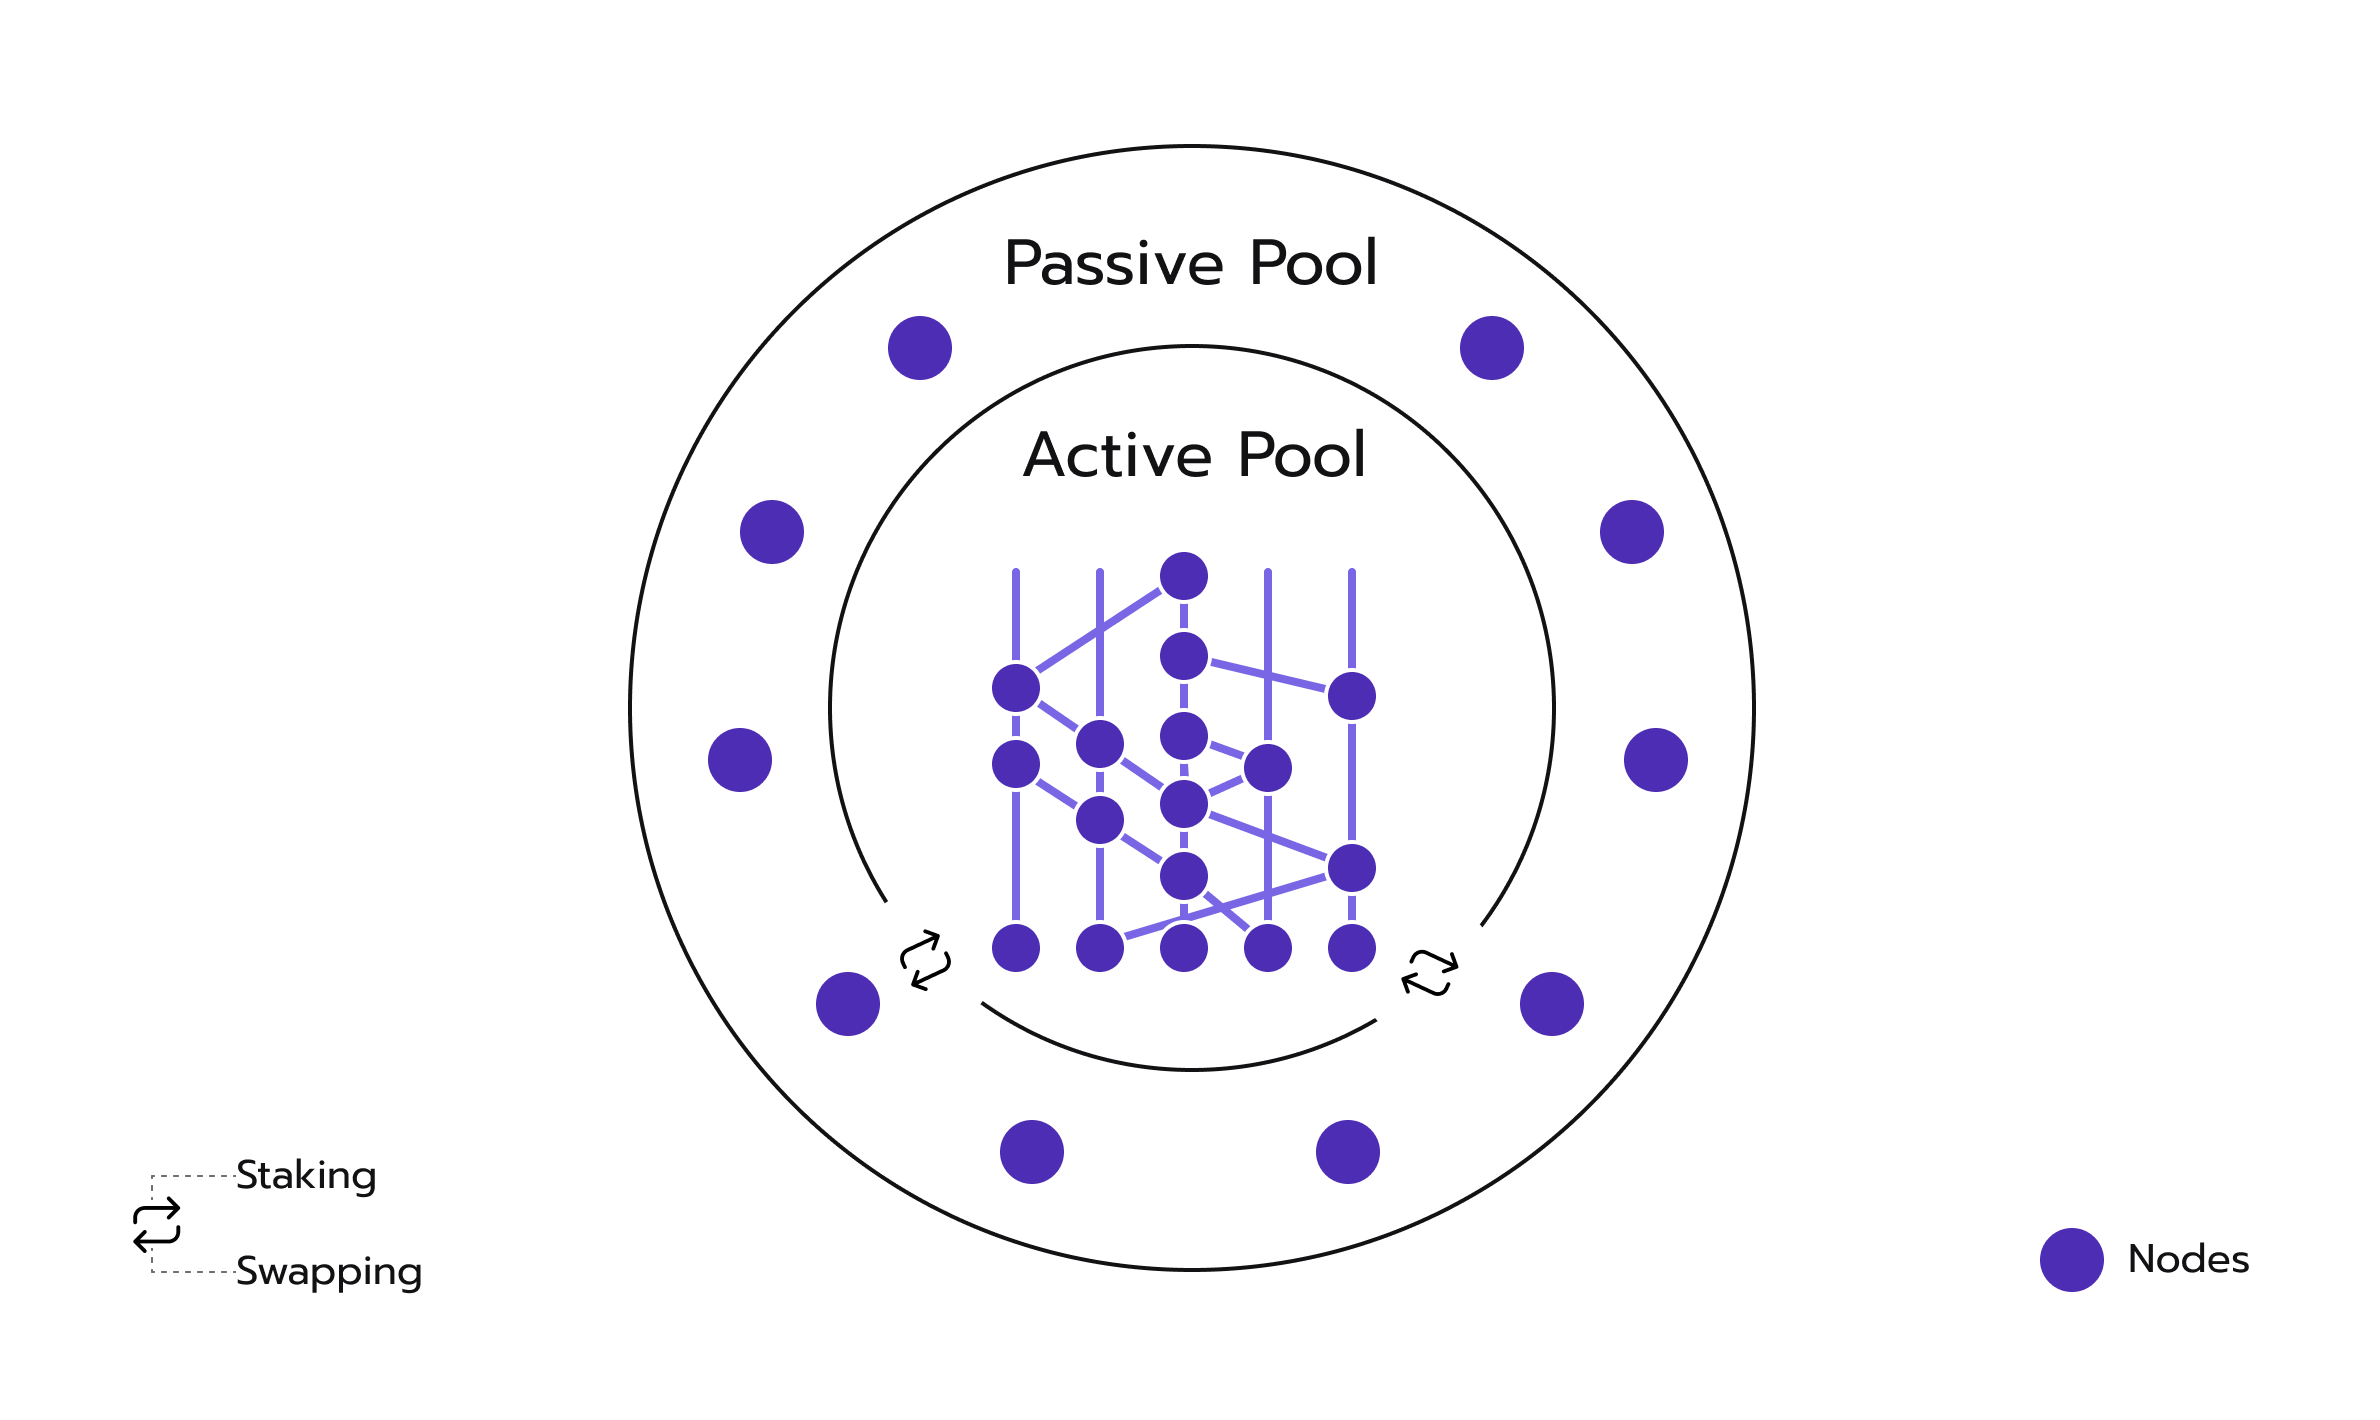
\includegraphics[width=1\textwidth]{figures/pools.png}
	\caption{Tagion is made up of 2 pools: an active pool of constant size where the consensus protocol takes place, and a passive pool of dynamic size.}
	\label{figure:pools}
\end{figure}

\subsection{Swapping}
    As the network runs, Tagion continuously swaps nodes between the active and the passive pool. A random node from the active pool is swapped with a random one from the passive pool after a fixed number of rounds (e.g. every 10\textsuperscript{th} round). The \gls{dart} is used to agree on an \acrfull{udr} choice. Optimally, nodes would have a precise agreement on when swapping occurs. But, due to the asynchronicity of the network, this cannot be guaranteed. If any node is significantly far behind the rest of the network, it might still receive messages from a node that the others have determined to be swapped out. The active pool is thus a local property, which might differ between nodes, though this would occur rarely in practise and for short durations. From a technical standpoint, leaving the active pool is straightforward, while joining is a slightly more complicated process. In rounds where a swap occurs, the nodes save the new active pool, and a set of \textit{foundations events} in the \gls{dart}. A joining node thus has a foundation it can built its own local Hashgraph on top of, and will quickly catch up to the rest of the active pool. The precise details for how nodes are \textit{randomly} chosen to be swapped is described in section \hyperref[sec:security]{\underline{5. Security}}.

\subsection{A Permissionless System}
    In summary, to avoid power accumulating on a small set of nodes, Tagion continuously swaps nodes between the passive and the active pool. Thus, power distribution is always changing, removing central points of control. Furthermore, Tagion's utilisation of 2 pools makes the system permissionless: any node can, without permission, join the network through the passive pool. These 2 attributes makes the Tagion a fully decentralised system.

\pagebreak